\section{Θεωρία Γράφων}
\selectlanguage{english}

\begin{figure}[ht]
    \begin{minipage}[c]{.46\linewidth}
        \centering
        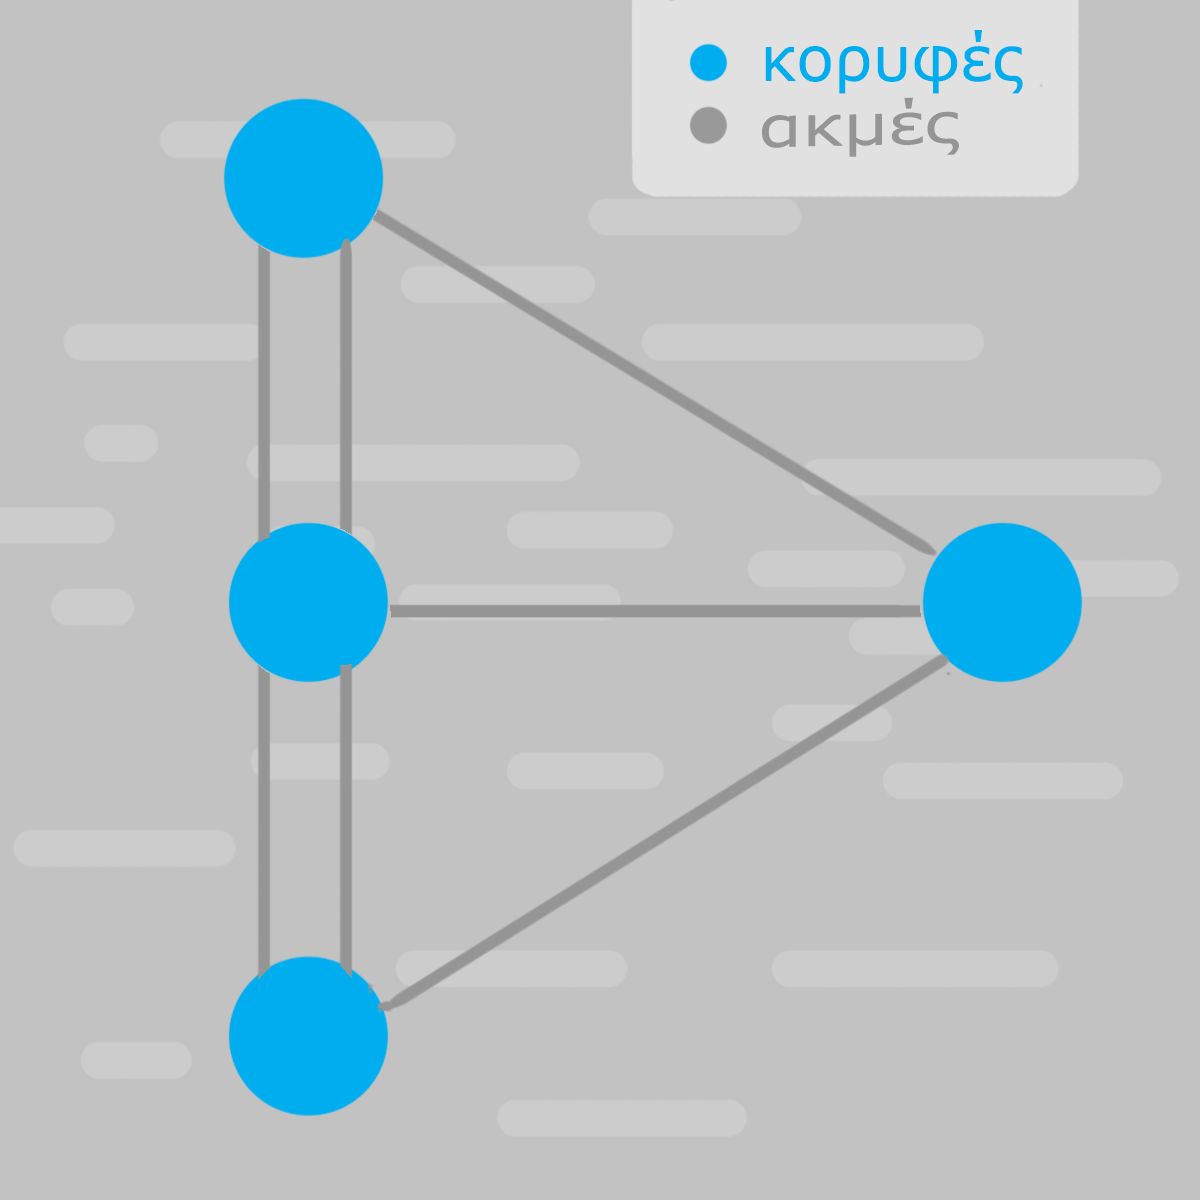
\includegraphics[scale=0.15]{2947_thesis/pictures/konigsberGraph.png}
        \caption{\lt{Königsberg} ως γράφος.}
        \label{3}
    \end{minipage}
    \hfill%
    \begin{minipage}[c]{.46\linewidth}
        \centering
        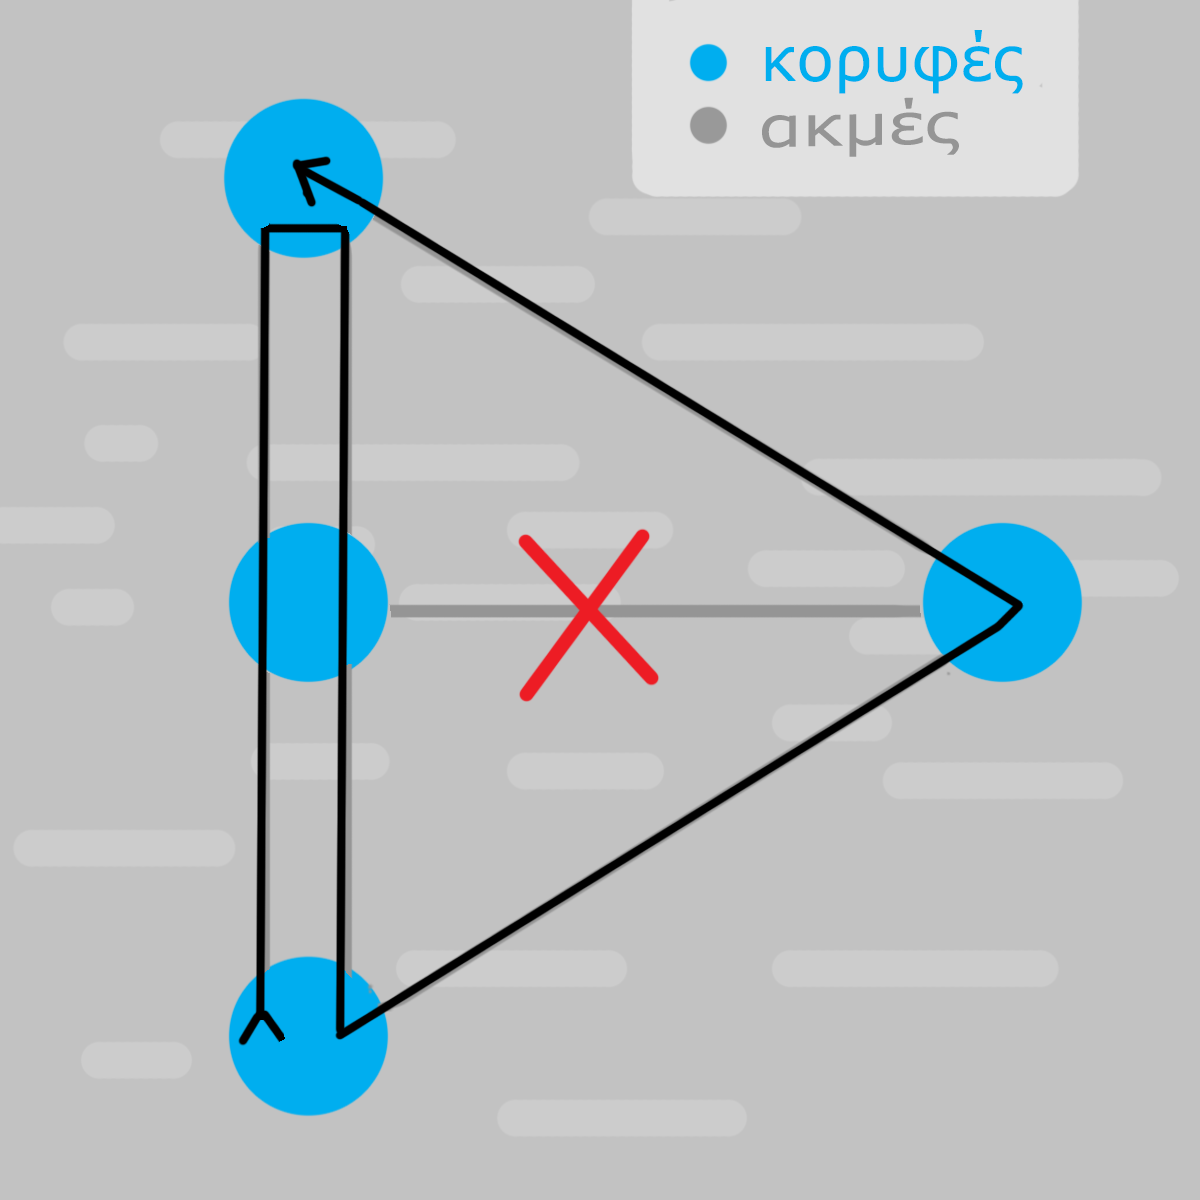
\includegraphics[scale=0.15]{2947_thesis/pictures/konigsbergEuler.png}
        \caption{Διαδρομή \lt{Euler}.}
        \label{4}
    \end{minipage}
\end{figure} 


\subsection{Εισαγωγή στην Θεωρία Γράφων}

Στην ουσία, ένας γράφος (\lt{graph}) είναι διάσπαρτα σημεία-κορυφές (\lt{vertices}) που ενώνονται με γραμμές-ακμές (\lt{edges}). Γράφους μπορούμε να συναντήσουμε σε διάφορα προβλήματα της καθημερινότητας όπως δίκτυα υποδομών (δίκτυο ύδρευσης), προβλήματα χαρτογράφησης (πλοήγηση), τηλεπικοινωνιών (δορυφόροι), μεταφορών (σιδηρόδρομοι), και άλλα \cite{manwlopoulos2014thewria}. Η θεωρία γράφων είναι ένας σημαντικός τομέας των μαθηματικών γιατί πέρα από το γεγονός ότι με χρήση αυτής μπορούμε να μοντελοποιήσουμε εύκολα προβλήματα της καθημερινότητας μας σε τομείς που αναφέρθηκαν παραπάνω, μπορούμε επίσης να αναπτύξουμε αλγόριθμους που λύνουν προβλήματα με χρήση γράφων. Παράδειγμα αυτού είναι και ο αλγόριθμος της αποικίας των μυρμηγκιών (\lt{Ant Colony Algorithm - ACO}) που θα αναλύσουμε σε αυτήν την πτυχιακή εργασία.

\subsection{Βασικοί Ορισμοί και έννοιες}
Για να γίνουν κατανοητά όσα θα αναφερθούν στην εργασία μας είναι απαραίτητο να παρουσιαστεί το θεωρητικό υπόβαθρο πάνω στο οποίο είναι βασισμένοι οι αλγόριθμοι βελτιστοποίησης. Για πιο αναλυτική μελέτη παραπέμπονται οι βιβλιογραφικές αναφορές που χρησιμοποιήθηκαν στο τέλος της εργασίας \cite{bondy1976usr, perez2020introduction, Gewrgiadis2017thewria, gkertsis2023thewria, mavrovouniotis2014ant, ntenisiwtis2023thewria}.

Ένας γράφος είναι μία μαθηματική δομή που ορίζεται με αυστηρό τρόπο μέσω δύο συνόλων: το σύνολο κορυφών (ή κόμβων, \lt{vertices}) και το σύνολο ακμών (ή γραμμών, \lt{edges}) που συνδέουν ζεύγη κορυφών μεταξύ τους και χρησιμοποιείται για την αναπαρά- σταση πληροφορίας σχετικά με συνδεσμολογία \cite{ntenisiwtis2023thewria}. Όταν δύο κορυφές είναι συνδεδεμένες, δηλαδή ενώνονται με τουλάχιστον μία ακμή ονομάζονται γειτονικές (\lt{adjacent vertices}) (για παράδειγμα στο \ref{5} η κορυφή "Α" και η κορυφή "Β" είναι γειτονικές), αντίστοιχα δύο ακμές που καταλήγουν σε ίδια κορυφή ονομάζονται προσπίπτουσες (\lt{incident edges}) της κορυφής αυτής. Το πλήθος των ακμών που προσπίπτουν σε μία κορυφή ονομάζεται βαθμός (\lt{degree}) ή αξία (\lt{valency}) της κορυφής αυτής. Τάξη (\lt{order}) ενός γράφου καλούμε το πλήθος των κορυφών που έχει (για παράδειγμα στο σχήμα \ref{5} η κορυφή "Ε" είναι τέταρτου βα- θμού και ο γράφος είναι έκτης τάξης). Ένας γράφος μπορεί να είναι είτε κατευθυνόμενος (\lt{directed graph}) όταν οι ακμές έχουν κατεύθυνση από μία κορυφή προς μία άλλη \ref{6}, είτε μη-κατευθυνόμενος (\lt{undirected graph}) όταν οι ακμές δεν έχουν κατεύθυνση και μπορούν να πηγαίνουν προς οπουδήποτε μεταξύ των κόμβων \ref{5} \cite{gkertsis2023thewria} \footnote{για περαιτέρω μελέτη: \lt{Directed and Undirected Graphs} από \lt{mathworks}\\ link: \url{https://www.mathworks.com/help/matlab/math/directed-and-undirected-graphs.html}}.

Στις ακμές (\lt{edges}) ενός γράφου μπορεί να γίνει επισύναψη βάρους (\lt{weight}), το οποίο αντιπροσωπεύει το κόστος, την απόσταση ή άλλες χρήσιμες πληροφορίες που συνδέονται με τις σχέσεις μεταξύ των κορυφών \lt{vertices}. Ένας γράφος που οι ακμές του έχουν συσχετι- στεί με έναν αριθμό ονομάζονται γράφος με βάρη (\lt{weighted graph}). Τα βάρη μπορούν να χρησιμοποιηθούν για την εκτέλεση αλγορίθμων βελτιστοποίησης και την αναζήτηση των βέλτιστων μονοπατιών σε γράφο \cite{ntenisiwtis2023thewria, gkertsis2023thewria}. Στον αλγόριθμο που θα αναλυθεί σε αυτήν την πτυχιακή εργασία τα βάρη αντιπροσωπεύουν την απόσταση (\lt{distance}) της διαδρομής ή το επίπεδο της φερομόνης (\lt{pheromone}) (θα αναλυθεί σε επόμενο κεφάλαιο).



\begin{figure}[ht]
    \begin{minipage}[c]{.46\linewidth}
        \centering
        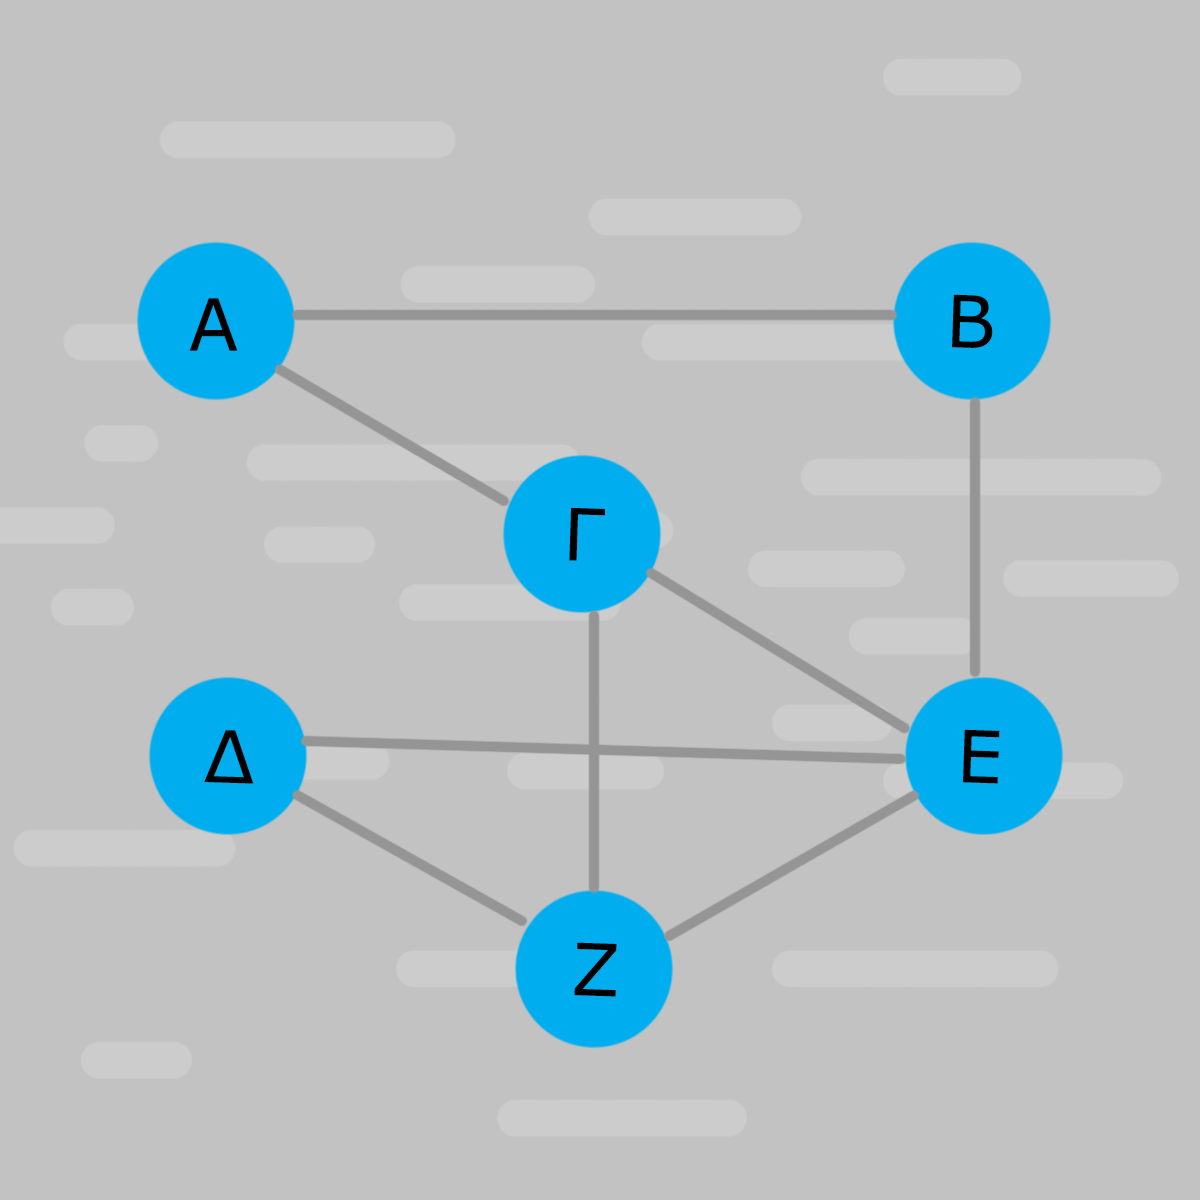
\includegraphics[scale=0.15]{2947_thesis/pictures/undirected.png}
        \caption{Μη κατευθυνόμενος γράφος.}
        \label{5}
    \end{minipage}
    \hfill%
    \begin{minipage}[c]{.46\linewidth}
        \centering
        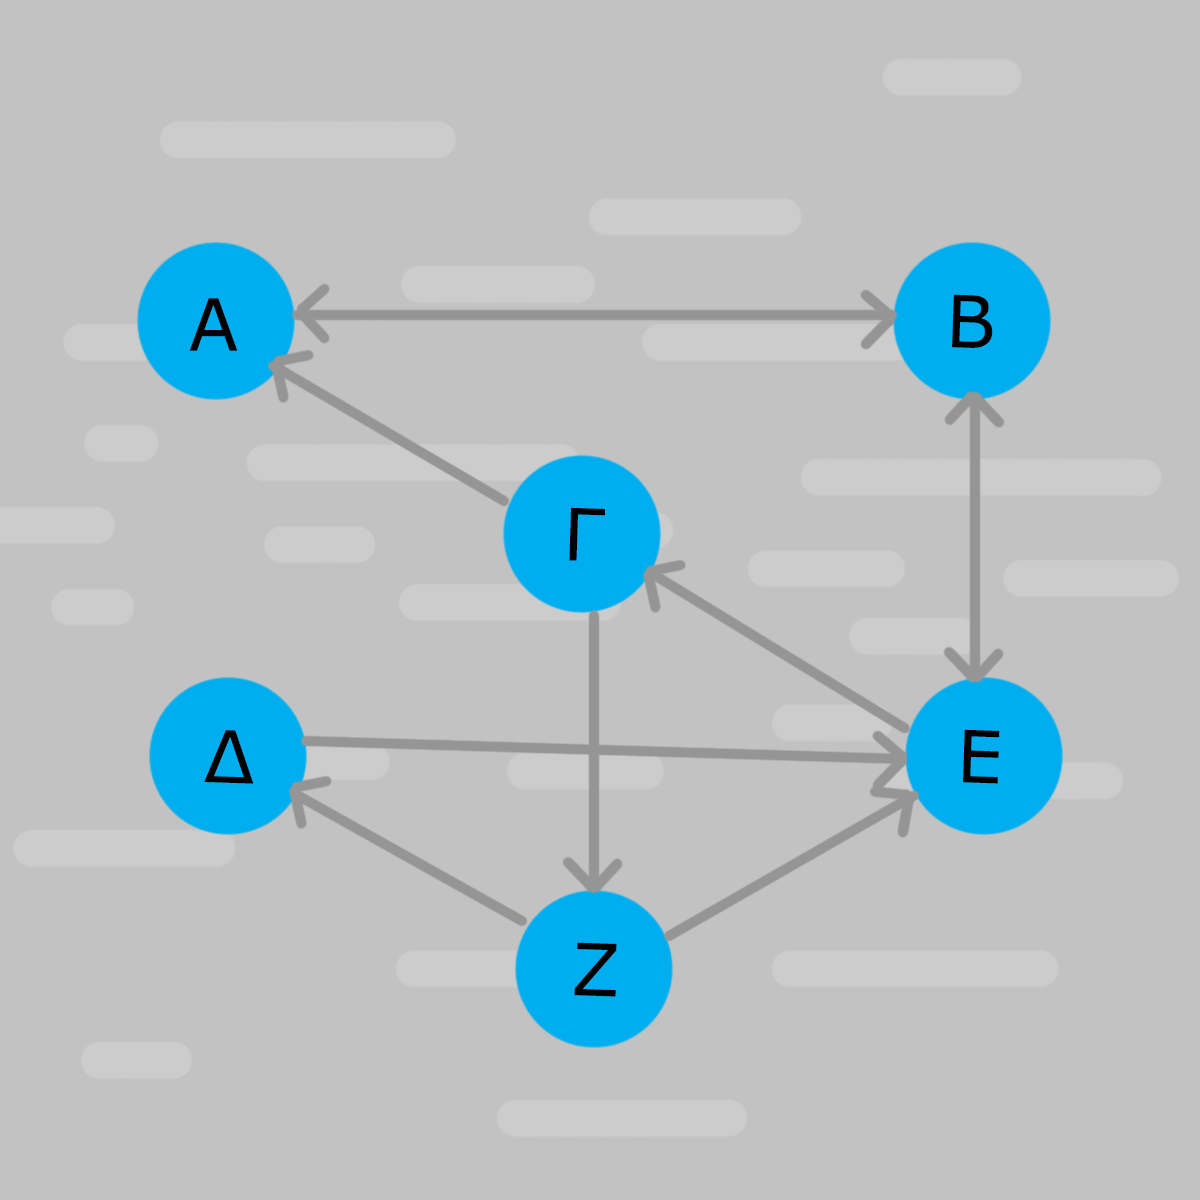
\includegraphics[scale=0.15]{2947_thesis/pictures/directed.png} 
        \caption{Κατευθυνόμενος γράφος.}
        \label{6}
    \end{minipage}
\end{figure}

\subsection{Μαθηματικό υπόβαθρο}
Ένας γράφος (\lt{Graph}) $G$ ορίζεται από δύο σύνολα $V(G)$ και $E(G)$. Το σύνολο $V(G)$ είναι ένα πεπερασμένο σύνολο, που περιέχει ως στοιχεία τις κορυφές (\lt{Vertices}) του γράφου. Το σύνολο $E(G)$ περιέχει τις ακμές (\lt{Edges}) ενός γράφου εκφρασμένες με σύνολα δύο γειτονικών κορυφών. Έτσι, πεπερασμένος (μη - κατευθυνόμενος, \lt{undirected}) γράφος, λέγεται το διατεταγμένο ζεύγος $G = (V(G), E(G))$ των πεπερασμένων συνόλων $V(G)$, $E(G)$ \cite{ntenisiwtis2023thewria}. Αν πάρουμε ως παράδειγμα τον γράφο $G$ στο \ref{7} παρατηρούμε ότι τα σύνολα $V(G)$ και $E(G)$ έχουν ως εξής: 
\begin{itemize}
  \item $V(G)=$[$v_1,v_2,v_3,v_4$]
  \item $E(G)=$[$e_1(v_1,v_2),e_2(v_1,v_3),e_3(v_2,v_3),e_4(v_3,v_4)$] 
\end{itemize}

\begin{figure}
    \centering
    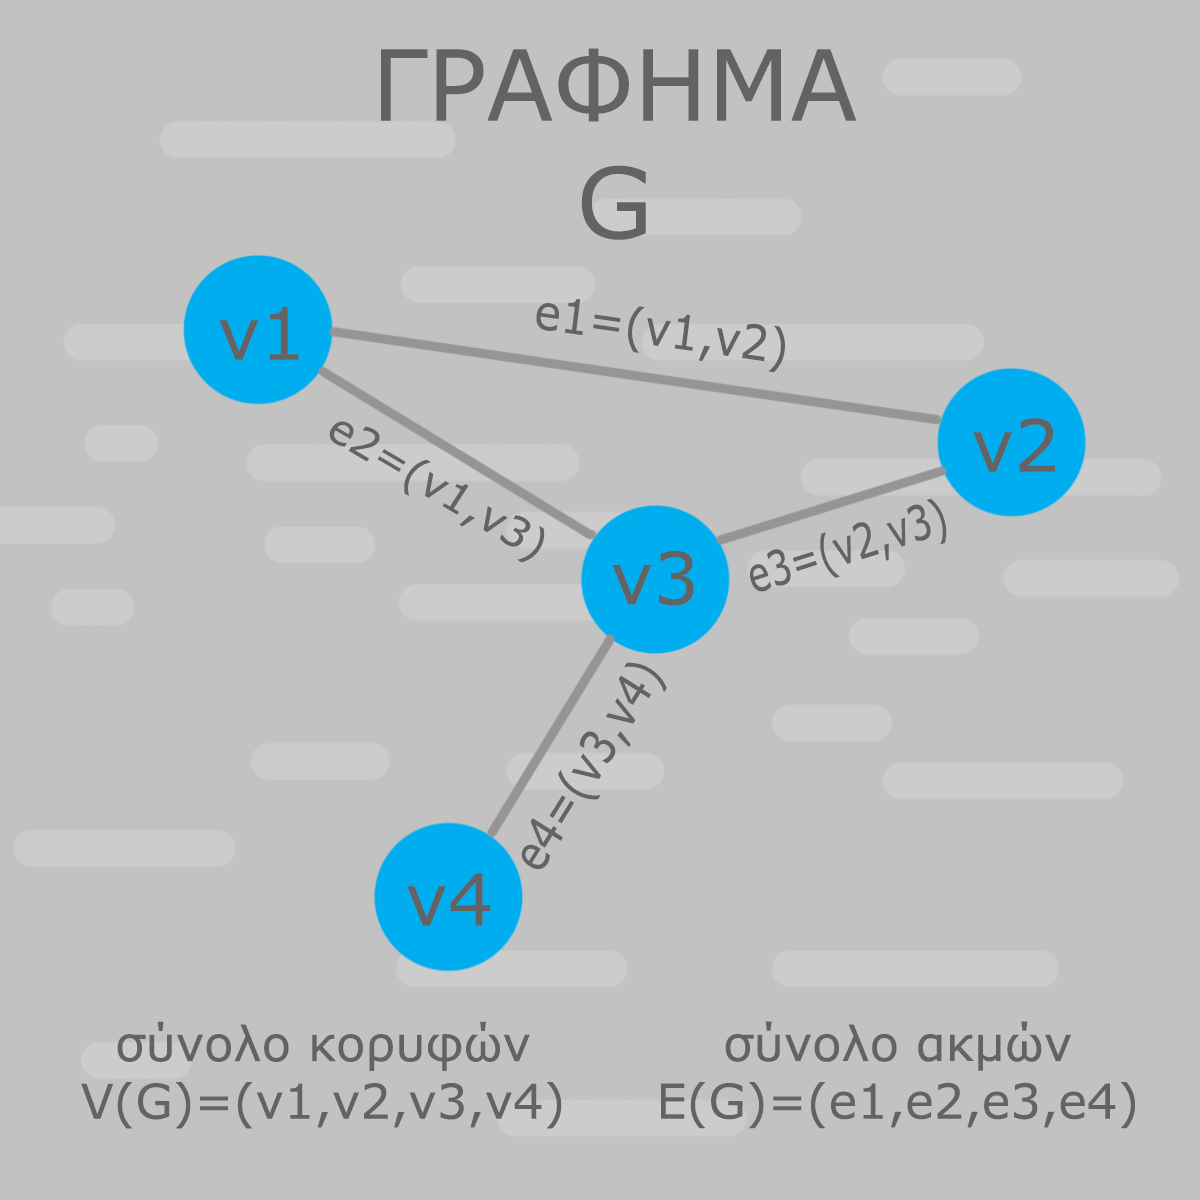
\includegraphics[scale=0.30]{2947_thesis/pictures/synola.png} 
    \caption{Σύνολα γραφήματος.}
    \label{7}
\end{figure}


\subsection{Αναπαράσταση γράφων}
Την κλασσική μορφή αναπαράστασης ενός γράφου την είδαμε ήδη παραπάνω, όπως φαίνεται στο σχήμα \ref{3}, όμως μια τέτοια αναπαράσταση δεν είναι καθόλου πρακτική σε προγραμματιστικό επίπεδο. Για αυτό αν θέλουμε να αναπαραστήσουμε γράφους σε έναν υπολογιστή χρησιμοποιούμε δομές δεδομένων. Οι δύο πιο βασικοί μέθοδοι αναπαράστασης γράφων σε υπολογιστές είναι οι πίνακες γειτνίασης (\lt{adjacency table}) και οι λίστες γειτνίασης (\lt{adjacency lists})\footnote{Αναπαράσταση γράφων, Παναγιώτα Φατούρου, Πανεπιστήμιο Κρήτης\\link: \url{https://www.csd.uoc.gr/~hy240/current/material/teacherClasses/Section10.pdf}}.

Πίνακα γειτνίασης (\lt{adjacency table}) ονομάζουμε ένα πίνακα μεγέθους $n\times n$, όπου $n$ ο αριθμός των κορυφών του γράφου. Κάθε κελί του πίνακα δείχνει την σχέση των αναγραφόμενων κορυφών. Σε ένα μη-κατευθυνόμενος γράφο το κελί $[i, j]$ παίρνει την τιμή 1 αν υπάρχει η ακμή $i \longleftrightarrow j$ και 0 αν δεν υπάρχει. 

Δηλαδή, έστω ο πίνακας γειτνίασης A του γράφου $G$:
\begin{center}
    $A[i, j] = 
    \begin{cases}
      1 & \text{αν $(i,j) \in E(G)$}\\
      0 & \text{αλλού}
    \end{cases}$
\end{center}
Είναι εύκολα αντιληπτό ότι ο πίνακας αυτός θα είναι συμμετρικός, δηλαδή ισούτε με τον ανάστροφό του, αφού η ακμή $i \longleftrightarrow j$ είναι ίδια με την ακμή $j \longleftrightarrow i$. Αντίστοιχα, σε έναν κατευθυνόμενο γράφο, το κελί $[i, j]$ παίρνει ομοίως τιμές 0 και 1 με την διαφορά ότι ο πίνακας δεν είναι συμμετρικός, οπότε η ακμή $i \rightarrow j \neq j \rightarrow i$. 

Οι πίνακες γειτνίασης μπορεί να έχουν και βάρη (\lt{weights}) που είναι μια επέκταση του απλού πίνακα γειτνίασης, σε αυτήν την περίπτωση, το έκαστο κελί ενός πίνακα, αντί για 1, περιέχει έναν αριθμό που ονομάζετε βάρος (\lt{weight}) και υποδηλώνει κάτι ανάλογα με την χρήση του. Σε έναν αλγόριθμο βελτιστοποίησης το βάρος μπορεί να υποδηλώνει την απόσταση της μιας κορυφής από την άλλη, την πιθανότητα επιλογής αυτής της διαδρομής, την επιρροή που δέχεται κάποια οντότητα σε επόμενο πιθανό πείραμα ή οποιοδήποτε άλλο κριτήριο που ανταποκρίνεται στον σκοπό του συγκεκριμένου αλγορίθμου\footnote{Πίνακες γειτνίασης, Παναγιώτα Φατούρου, Πανεπιστήμιο Κρήτης \\link: \url{https://www.csd.uoc.gr/~hy240/current/material/teacherClasses/Section10.pdf}} \cite{gkertsis2023thewria}.


Για παράδειγμα στο σχήμα \ref{7}, πρόκειται για έναν μη-κατευθυνόμενο γράφο χωρίς βάρη με 4 κορυφές, δηλαδή $n=4$ και με ακμές που φαίνονται στο σύνολο $E(G)$. Επομένως ο πίνακας γειτνίασης του διαμορφώνεται έτσι: 
$$
G_{n,n} = 
\begin{array}{c|c c c c}
   & v_{1} & v_{2} & v_{3} & v_{4} \\ \hline
   v_{1} & v_{1,1} & v_{1,2} & v_{1,3} & v_{1,4} \\
   v_{2} & v_{2,1} & v_{2,2} &   v_{2,3} & v_{2,4} \\
   v_{3} & v_{3,1} & v_{3,2} & v_{3,3} & v_{3,4} \\
   v_{4} & v_{4,1} & v_{4,2} & v_{4,3} & v_{4,4} 
\end{array}
$$
που αντικαθιστώντας 0-1 προκύπτει: 
$$
G_{4,4} = 
\begin{array}{c|c c c c}
   & v_{1} & v_{2} & v_{3} & v_{4} \\ \hline
   v_{1} & 0 & 1 & 1 & 0 \\
   v_{2} & 1 & 0 & 1 & 0 \\
   v_{3} & 1 & 1 & 0 & 1 \\
   v_{4} & 0 & 0 & 1 & 0 
\end{array}
$$
όπου 1 συμβολίζει ότι αυτές οι δύο κορυφές είναι γειτονικές έχοντας ακμή να τις ενώνει, ενώ 0 ότι δεν υπάρχει ακμή.

Λίστα γειτνίασης (\lt{adjacency list}) ονομάζουμε μια αναπαράσταση γράφων όπου για κάθε κορυφή διατηρείται μια λίστα των γειτόνων της. Σε περίπτωση κατευθυνόμενου γράφου μπορεί να υπάρχει ξεχωριστή λίστα για τους εξερχόμενους και τους εισερχόμενους γείτονες-κορυφές. Αυτή η αναπαράσταση αποκτά αξία σε γράφους με αραιή (\lt{sparse}) συνδεσιμότητα αφού γίνεται εξοικονόμηση μνήμης\footnote{Λίστες Γειτνίασης, Παναγιώτα Φατούρου, Πανεπιστήμιο Κρήτης \\link: \url{https://www.csd.uoc.gr/~hy240/current/material/teacherClasses/Section10.pdf}}.

Το πόσο μεγάλη θα είναι η λίστα εξαρτάται από τον αριθμό των κορυφών του γράφου. Κάθε στοιχείο στην λίστα συμβολίζει μία ακμή του γράφου. Στην περίπτωση ενός μη-κατευθυνόμενου γράφο, η λίστα γειτνίασης για κάθε κορυφή περιλαμβάνει τους γείτονές της, δηλαδή τις άλλες κορυφές με τις οποίες συνδέεται με μια ακμή. Αν υπάρχουν $n$ κορυφές στον γράφο, η λίστα γειτνίασης για κάθε κορυφή περιλαμβάνει μια λίστα με το πλήθος των γειτόνων της. Για παράδειγμα στο σχήμα \ref{7} που απεικονίζεται ένας μη-κατευθυνόμενος γράφος με 4 κορυφές, άρα $n=4$ και ακμές που φαίνονται στο σύνολο $E(G)$ του αντίστοιχου σχήματος, αν η αναπαράσταση γινόταν με λίστα γειτνίασης θα ήταν ως εξής: 
\begin{enumerate}
    \item $v_1: \{v_2, v_3\}$
    \item $v_2: \{v_1, v_3\}$
    \item $v_3: \{v_1, v_2, v_4\}$
    \item $v_4: \{v_3\}$
\end{enumerate}

Στην περίπτωση ενός κατευθυνόμενου γράφου, σε κάθε κορυφή θα υπάρχαν 2 λίστες, μία που εκφράζει τις προηγούμενες κορυφές και μία που εκφράζει τις ακόλουθες. Για παράδειγμα στο σχήμα \ref{6} η λίστα γειτνίασης θα αναπαριστόταν ως εξής: 
\begin{enumerate}
    \item Α: προηγούμενοι:$\{B, Γ\}$, ακόλουθοι:$\{B\}$
    \item Β: προηγούμενοι:$\{A, E\}$, ακόλουθοι:$\{A, E\}$
    \item Γ: προηγούμενοι:$\{E\}$, ακόλουθοι:$\{A, Z\}$
    \item Δ: προηγούμενοι:$\{Z\}$, ακόλουθοι:$\{E\}$
    \item Ε: προηγούμενοι:$\{Δ, Z\}$, ακόλουθοι:$\{B, Γ\}$
    \item Ζ: προηγούμενοι:$\{Γ\}$, ακόλουθοι:$\{Δ, E\}$
    
\end{enumerate}


Σε σχέση με τους πίνακες γειτνίασης, οι λίστες γειτνίασης επιτρέπουν την εύκολη πρό- σβαση στα δεδομένα του γράφου καθώς και τροποποίηση αυτών, δηλαδή η εισαγωγή και η διαγραφή μιας κορυφής μπορεί να γίνει με ευκολία. Επίσης σε αραιούς γράφους (δηλαδή γράφους με λίγες ακμές) απαιτούν λιγότερη μνήμη, ενώ σε πλήρη συνδεδεμένους γράφους περισσότερη. Αντίθετα, οι πίνακες γειτνίασης δεν επιτρέπουν εύκολη τροποποίηση στις κορυφές και τις σχέσεις μεταξύ τους, ούτε εύκολη εισαγωγή και διαγραφή, για παράδειγμα μία πιθανή εισαγωγή θα προκαλέσει αύξηση στο μέγεθος του πίνακα\footnote{Θετικά και Αρνητικά, Παναγιώτα Φατούρου, Πανεπιστήμιο Κρήτης \\link: \url{https://www.csd.uoc.gr/~hy240/current/material/teacherClasses/Section10.pdf}}. Όμως, το γεγονός ότι πολλές λειτουργίες μπορούν απλά και αποτελεσματικά να μοντελοποιηθούν τους κάνει ιδανικούς για χρήση στον αλγόριθμο μας. 
